\documentclass[border=7pt]{standalone}
\usepackage{amsmath,amssymb,bm,mathtools}
\usepackage[fontset=none]{ctex}
\setCJKmainfont{Songti SC}\setCJKsansfont{PingFang SC}
\usepackage{tikz}\usetikzlibrary{arrows.meta,calc,patterns,angles,quotes,decorations.markings,decorations.pathmorphing}
\newcommand{\dd}{\mathop{}\!\mathrm d}
\definecolor{blue}{HTML}{235789}\definecolor{red}{HTML}{BC4B41}
\tikzset{axis/.style={->,>=Stealth,line width=.55pt},world/.style={line width=.9pt},flow/.style={->,>=Stealth,line width=.85pt},ray/.style={->,>=Stealth,line width=.85pt},guide/.style={dashed,line width=.4pt},aux/.style={dashed,line width=.4pt},dim/.style={<->,>=Stealth,line width=.5pt},every node/.style={font=\normalsize},force/.style={->,>=Stealth,very thick},gas/.style={fill=blue!7}}
\begin{document}
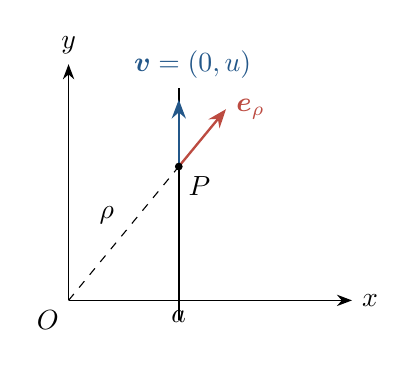
\begin{tikzpicture}
\draw[axis](0,0)--(3.6,0)node[right]{$x$};\draw[axis](0,0)--(0,3)node[above]{$y$};
\draw[world](1.4,-.25)--(1.4,2.7);\coordinate(P)at(1.4,1.7);
\draw[guide](0,0)--(P)node[midway,above left]{$\rho$};
\draw[flow,blue](P)--++(0,.85)node[above,xshift=5pt,yshift=4pt]{$\bm v=(0,u)$};
\draw[flow,red](P)--++(.6,.7286)node[right]{$\bm e_\rho$};
\fill(P)circle(1.4pt)node[below right]{$P$};\node[below]at(1.4,0){$a$};\node[below left]at(0,0){$O$};
\end{tikzpicture}
\end{document}
